\documentclass[]{article}
\usepackage{xcolor}
\usepackage{listings}
\usepackage{showexpl}
\usepackage{graphicx}
\usepackage[bahasai]{babel}
\lstset{language=SQL,
	 numbers=left,
		stepnumber=1,
	numberstyle=\ttfamily,
	basicstyle=\ttfamily,
	keywordstyle=\color{blue}\ttfamily,
	stringstyle=\color{red}\ttfamily,
	commentstyle=\color{gray}\ttfamily,
	morecomment=[l][\color{magenta}]{\#},
    breaklines=true,
    %postbreak=\mbox{\textcolor{red}{$\hookrightarrow$}\space}
}


%opening
\title{Laporan Praktikum 2: Query}
\author{Akhmad Thoriq Afif NRP 5024201028}

\begin{document}
\maketitle
\section{Deskripsi Tugas}
Mengerjakan soal latihan yang terdapat pada https://www.sql-practice.com/ dengan minimal pengerjaan level 'Easy'. Kemudian membuat laporan dari hasil pengerjaan tersebut. 
\section{Jawaban}
\subsection{Easy 1}
Show first name, last name, and gender of patients who's gender is 'M'
\lstinputlisting[label={maxvalue},caption={Easy-1}, language={SQL}]{easy-1.sql}
\begin{figure}[H]
    \centering
    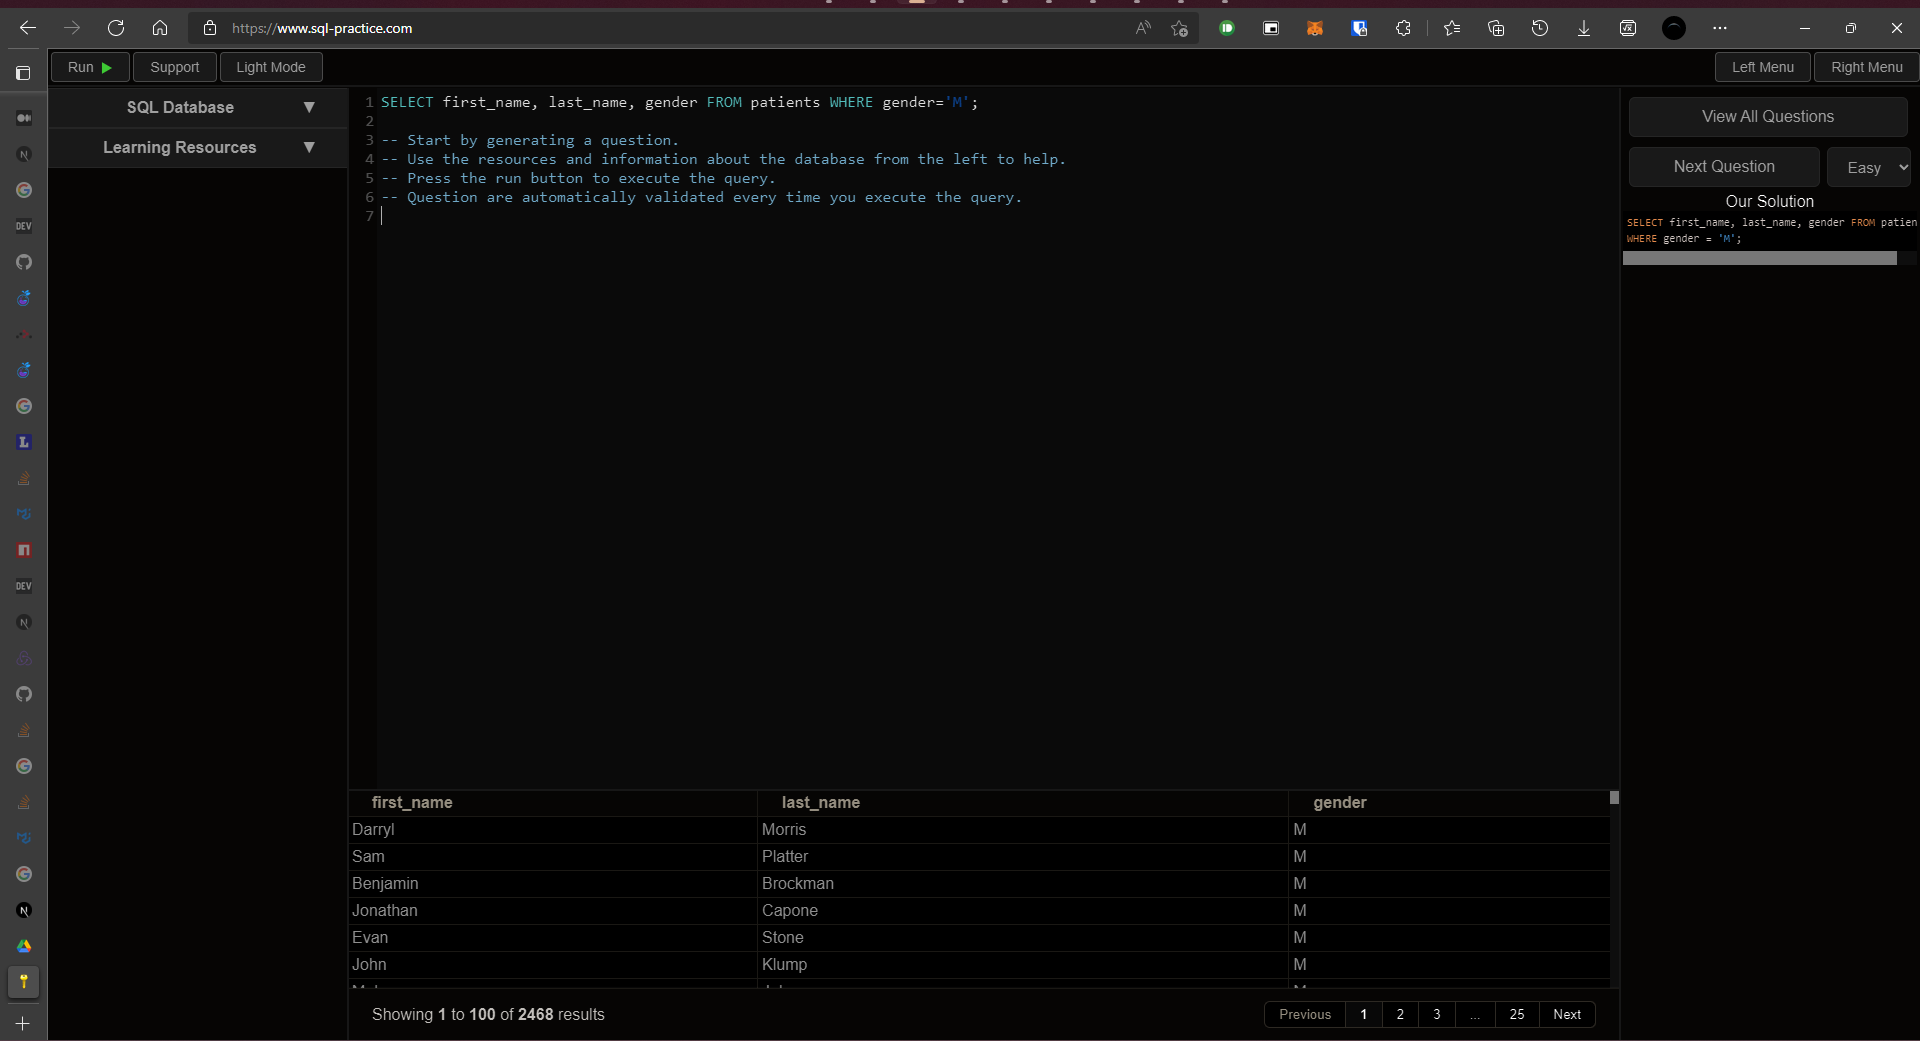
\includegraphics[width=12cm]{easy-1.png}
    \caption{Hasil Query Soal Easy 1}
\end{figure}
\subsection{Easy 2}
Show first name and last name of patients who does not have allergies (null).
\lstinputlisting[label={maxvalue},caption={Easy-2}, language={SQL}]{easy-2.sql}
\begin{figure}[H]
    \centering
    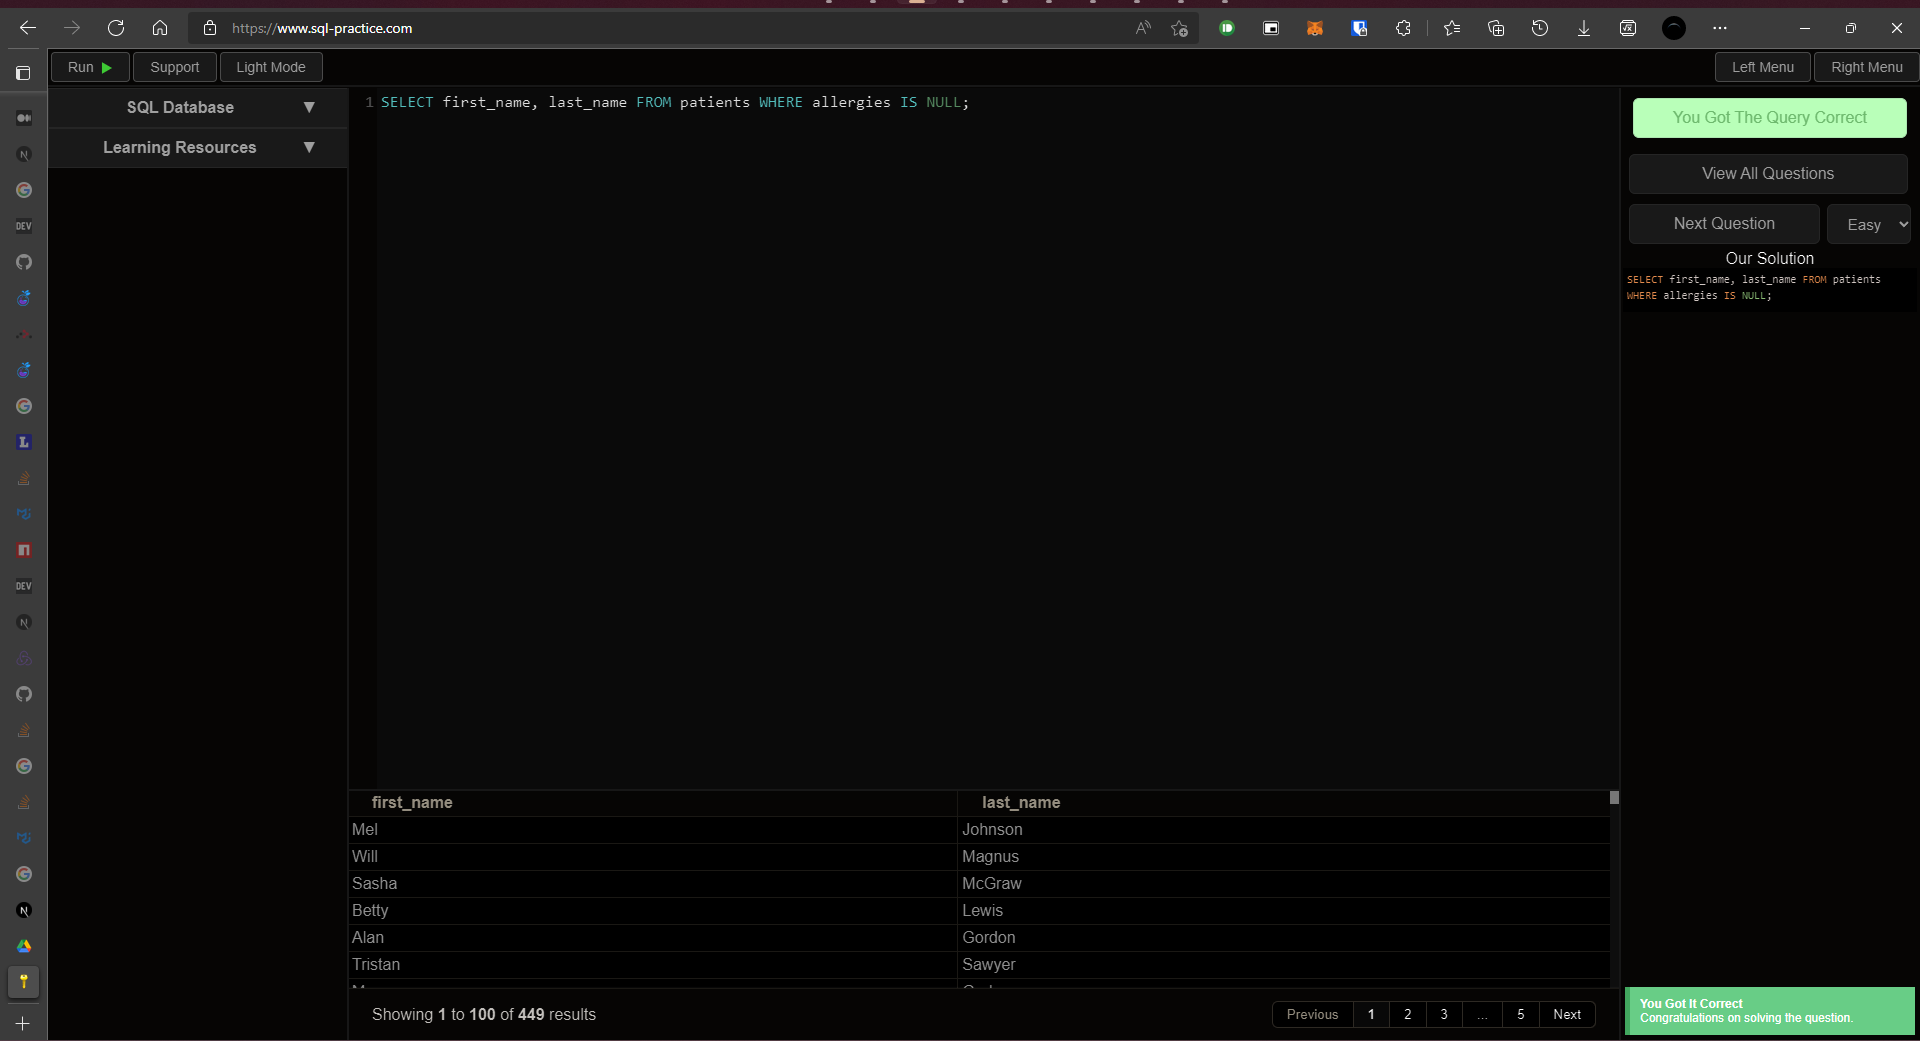
\includegraphics[width=12cm]{easy-2.png}
    \caption{Hasil Query Soal Easy 2}
\end{figure}
\subsection{Easy 3}
Show first name of patients that start with the letter 'C'
\lstinputlisting[label={maxvalue},caption={Easy-3}, language={SQL}]{easy-3.sql}
\begin{figure}[H]
    \centering
    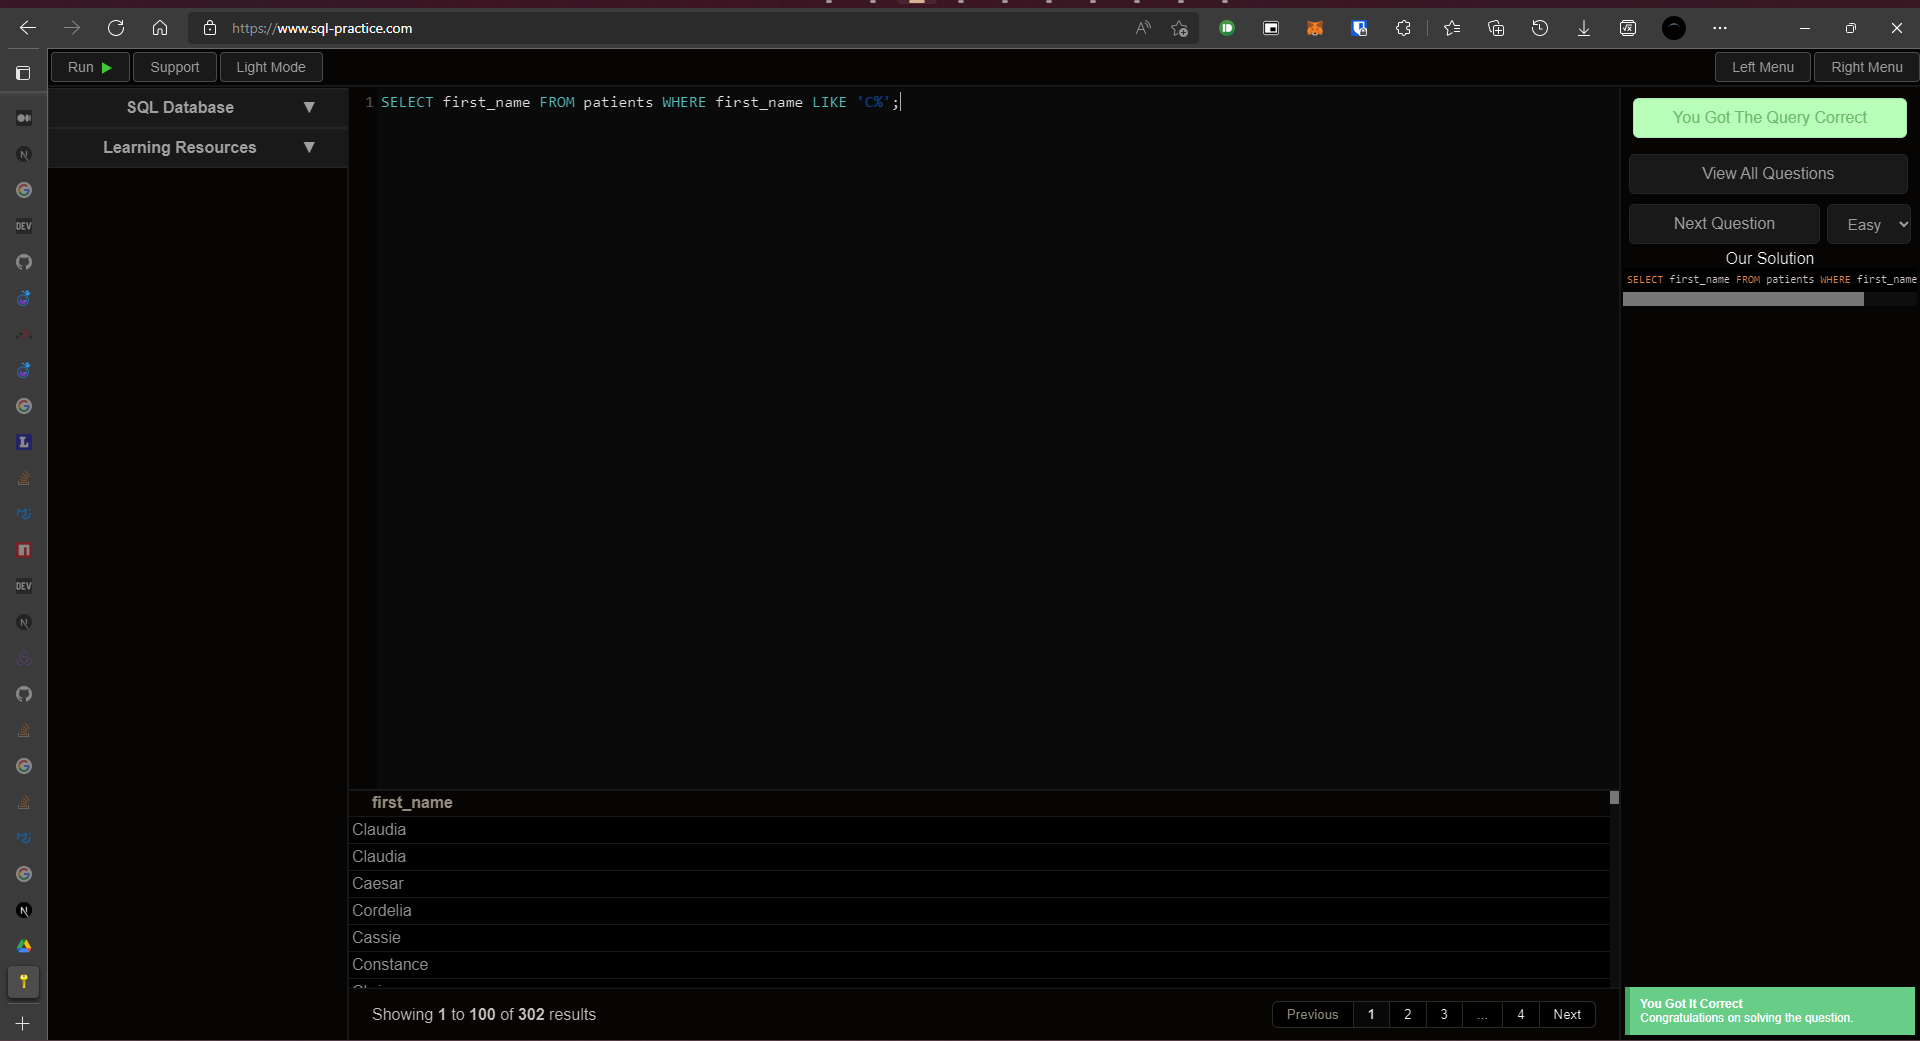
\includegraphics[width=12cm]{easy-3.png}
    \caption{Hasil Query Soal Easy 3}
\end{figure}
\subsection{Easy 4}
Show first name and last name of patients that weight within the range of 100 to 120 (inclusive)
\lstinputlisting[label={maxvalue},caption={Easy-4}, language={SQL}]{easy-4.sql}
\begin{figure}[H]
    \centering
    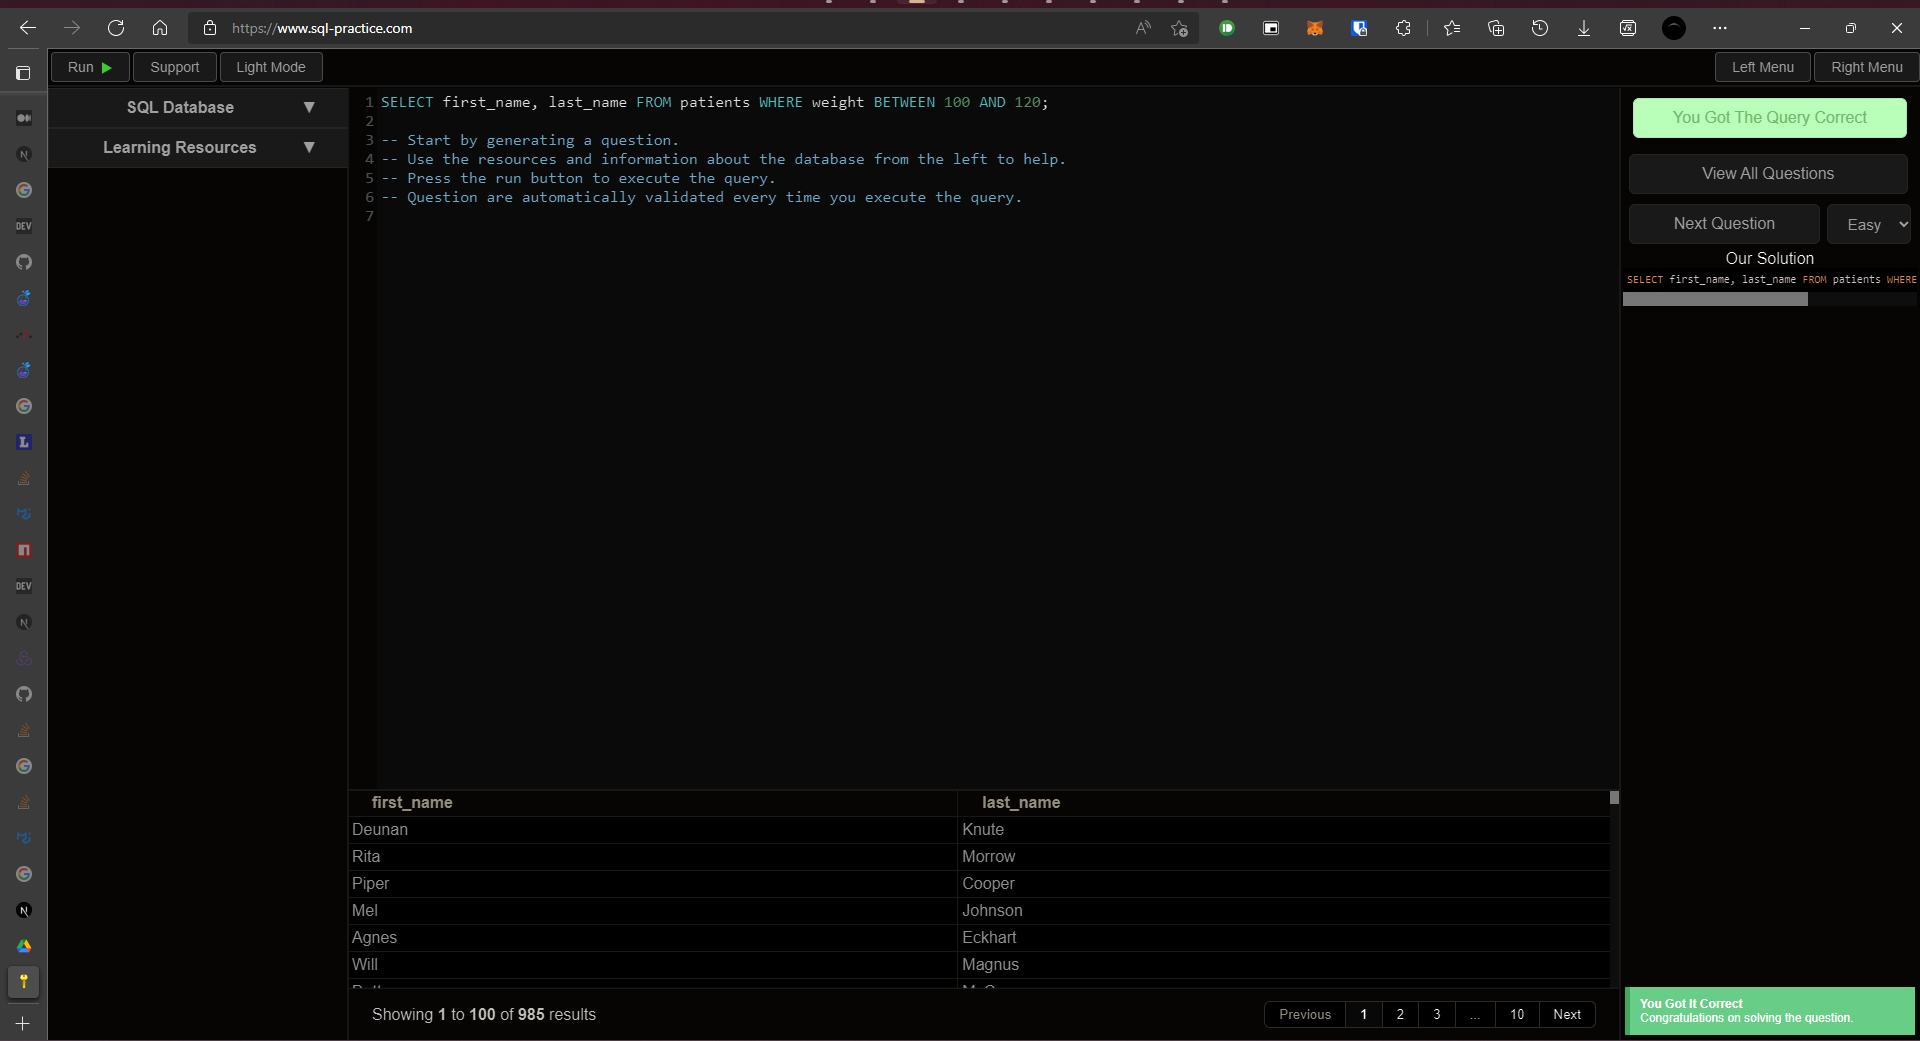
\includegraphics[width=12cm]{easy-4.png}
    \caption{Hasil Query Soal Easy 4}
\end{figure}
\subsection{Easy 5}
Update the patients table for the allergies column. If the patient's allergies is null then replace it with 'NKA'
\lstinputlisting[label={maxvalue},caption={Easy-5}, language={SQL}]{easy-5.sql}
\begin{figure}[H]
    \centering
    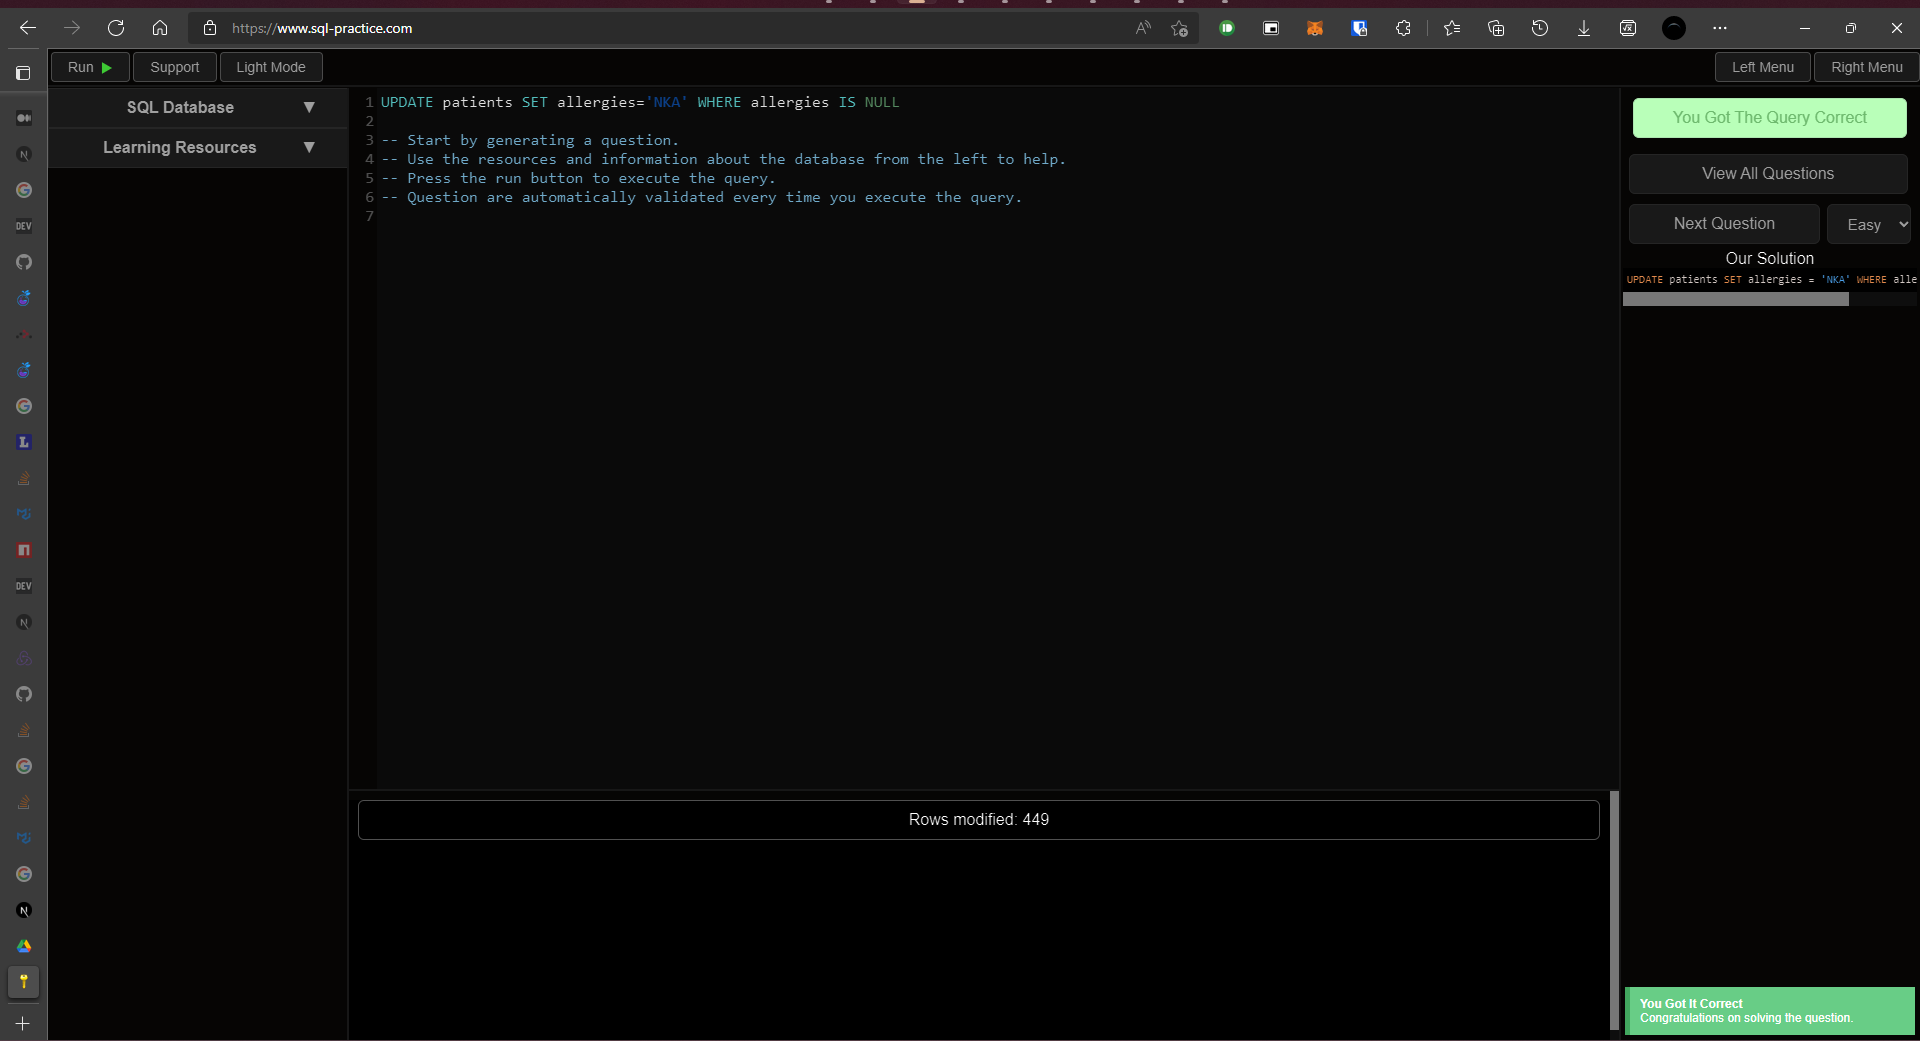
\includegraphics[width=12cm]{easy-5.png}
    \caption{Hasil Query Soal Easy 5}
\end{figure}
\subsection{Easy 6}
Show first name and last name concatinated into one column to show their full name.
\lstinputlisting[label={maxvalue},caption={Easy-6}, language={SQL}]{easy-6.sql}
\begin{figure}[H]
    \centering
    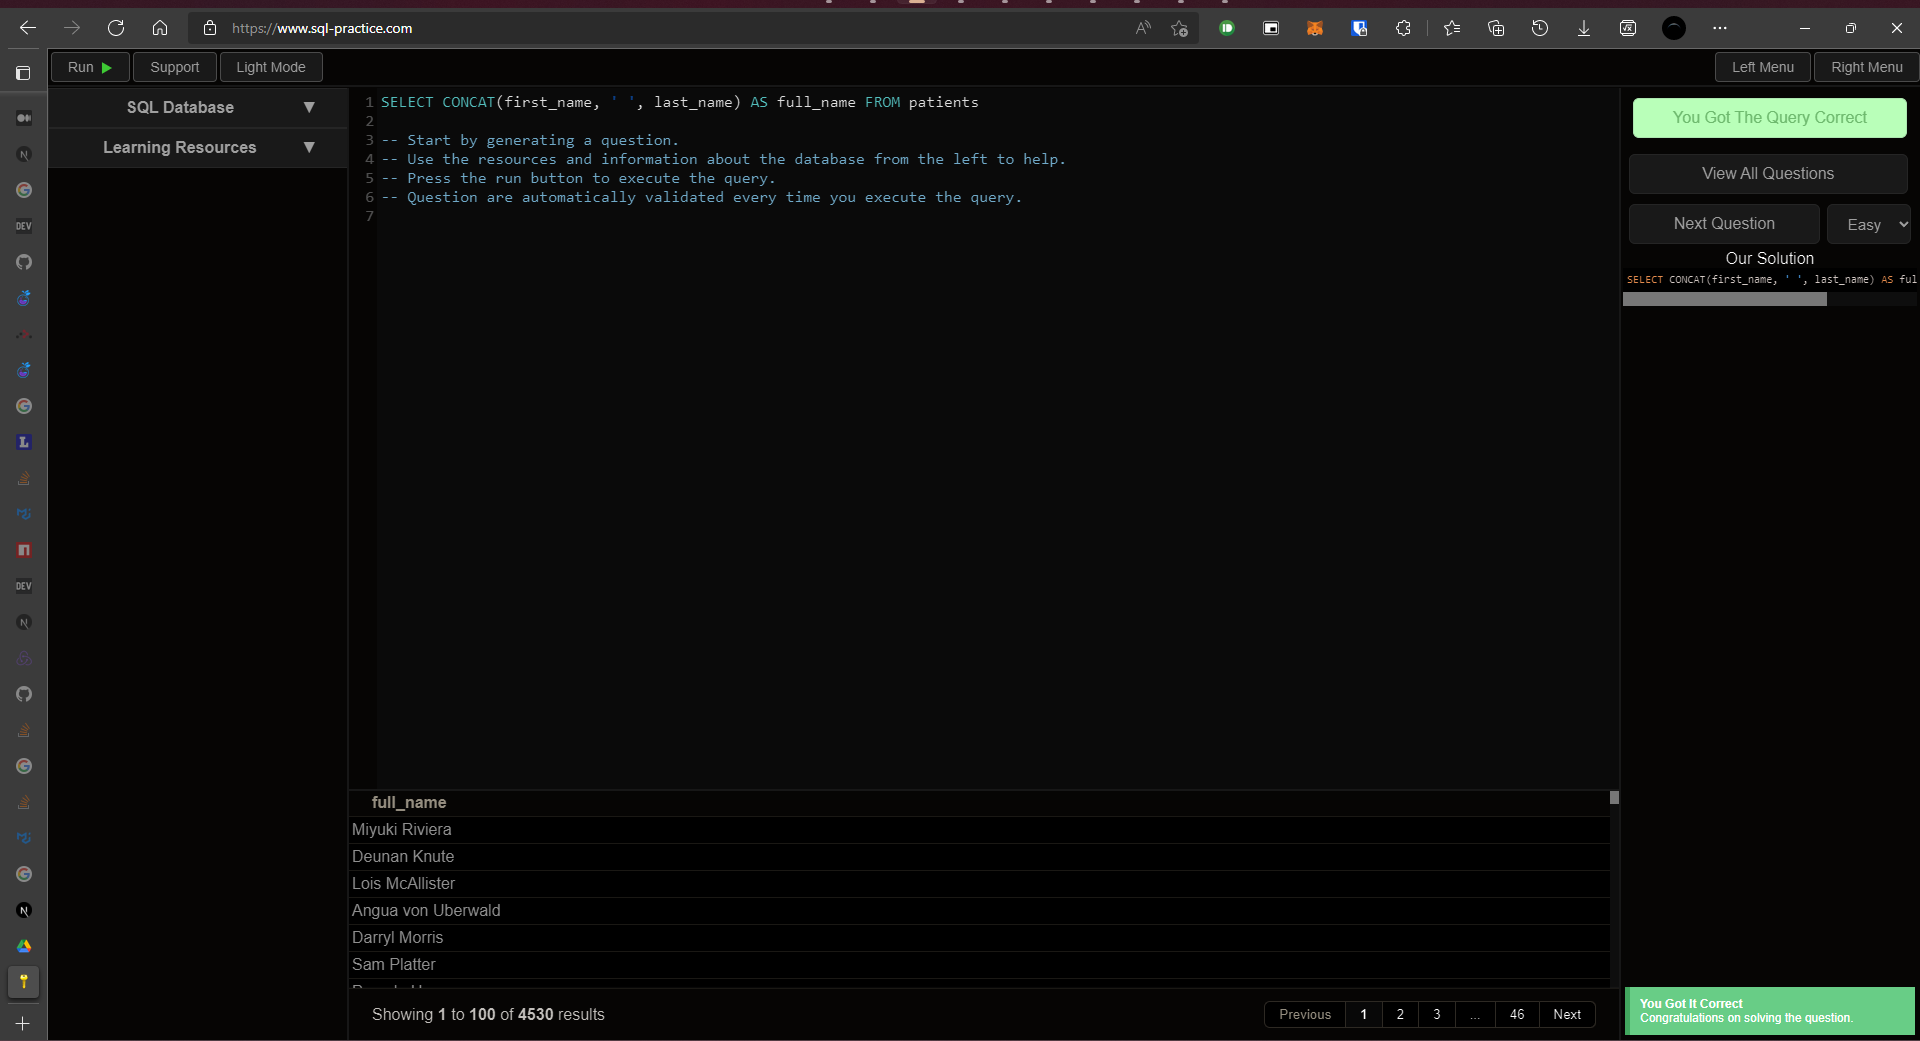
\includegraphics[width=12cm]{easy-6.png}
    \caption{Hasil Query Soal Easy 6}
\end{figure}
\subsection{Easy 7}
Show first name, last name, and the full province name of each patient. Example: 'Ontario' instead of 'ON'
\lstinputlisting[label={maxvalue},caption={Easy-7}, language={SQL}]{easy-7.sql}
\begin{figure}[H]
    \centering
    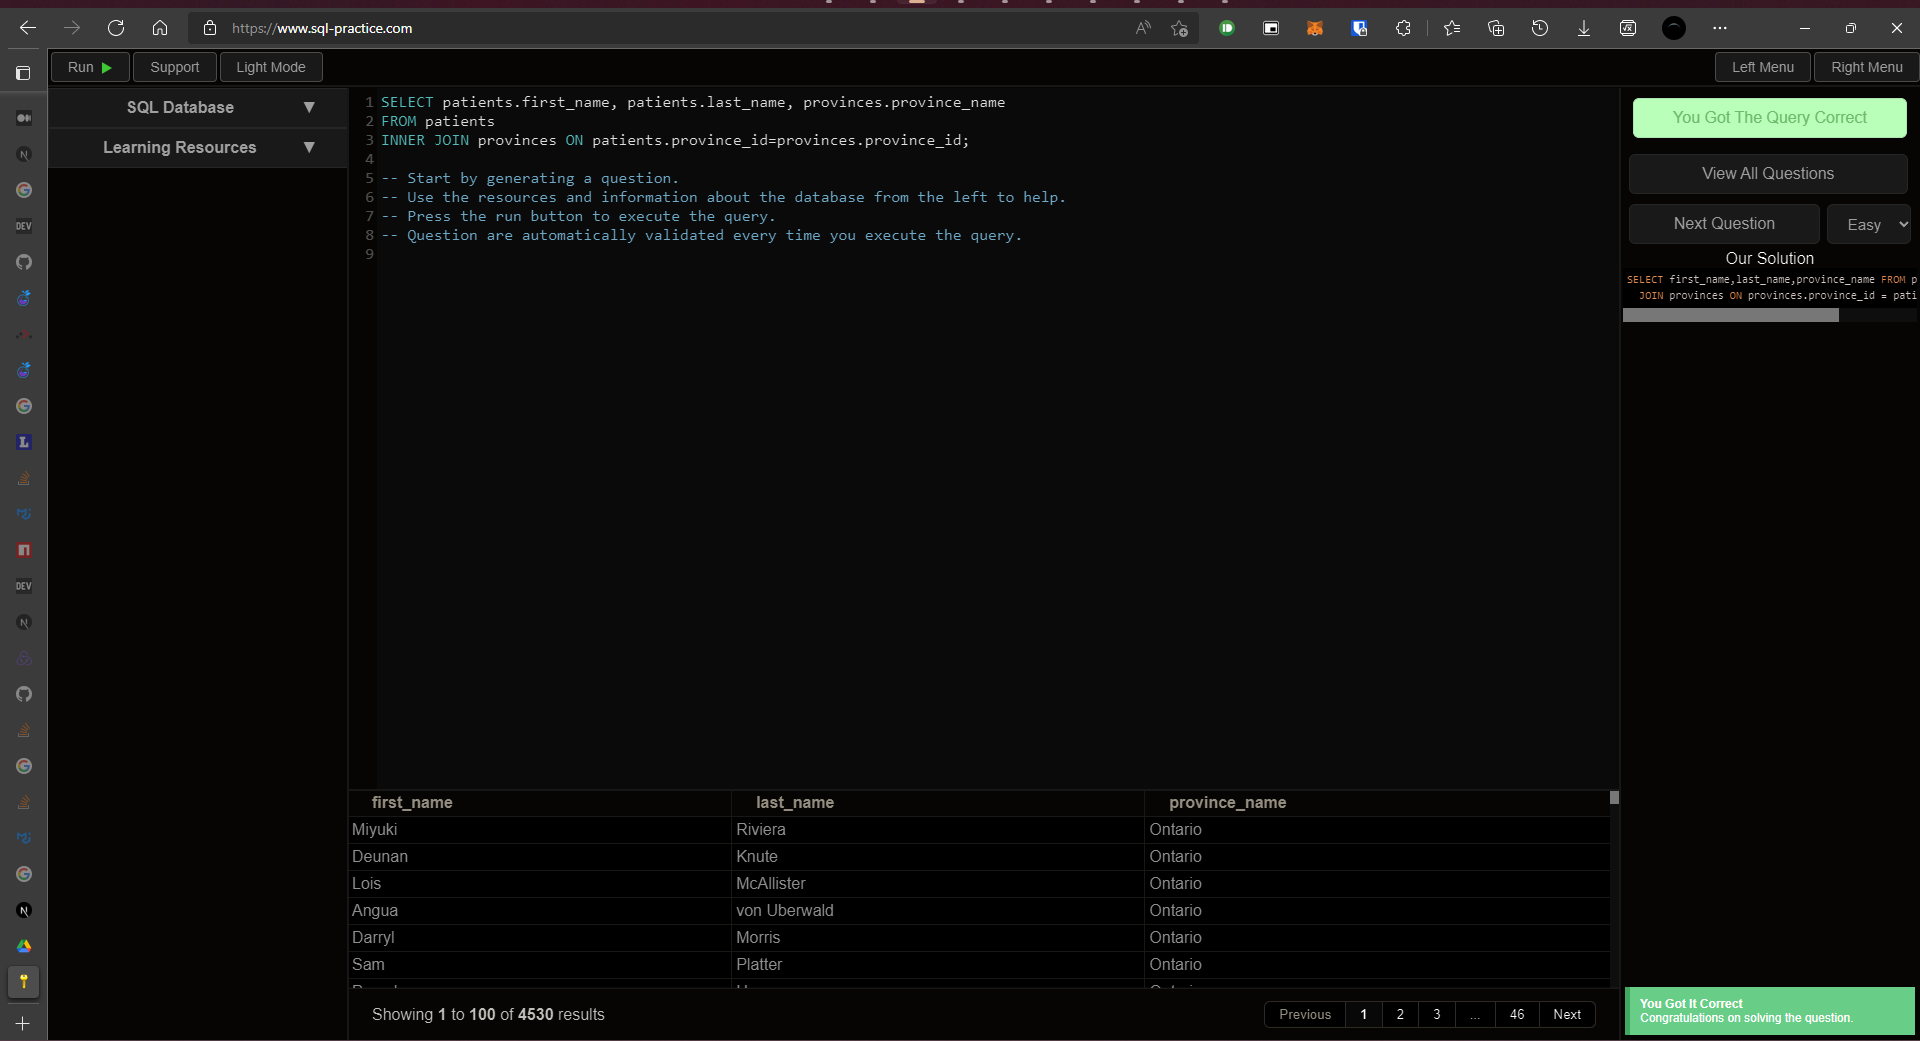
\includegraphics[width=12cm]{easy-7.png}
    \caption{Hasil Query Soal Easy 7}
\end{figure}
\subsection{Easy 8}
Show how many patients have a birth\_date with 2010 as the birth year.
\lstinputlisting[label={maxvalue},caption={Easy-8}, language={SQL}]{easy-8.sql}
\begin{figure}[H]
    \centering
    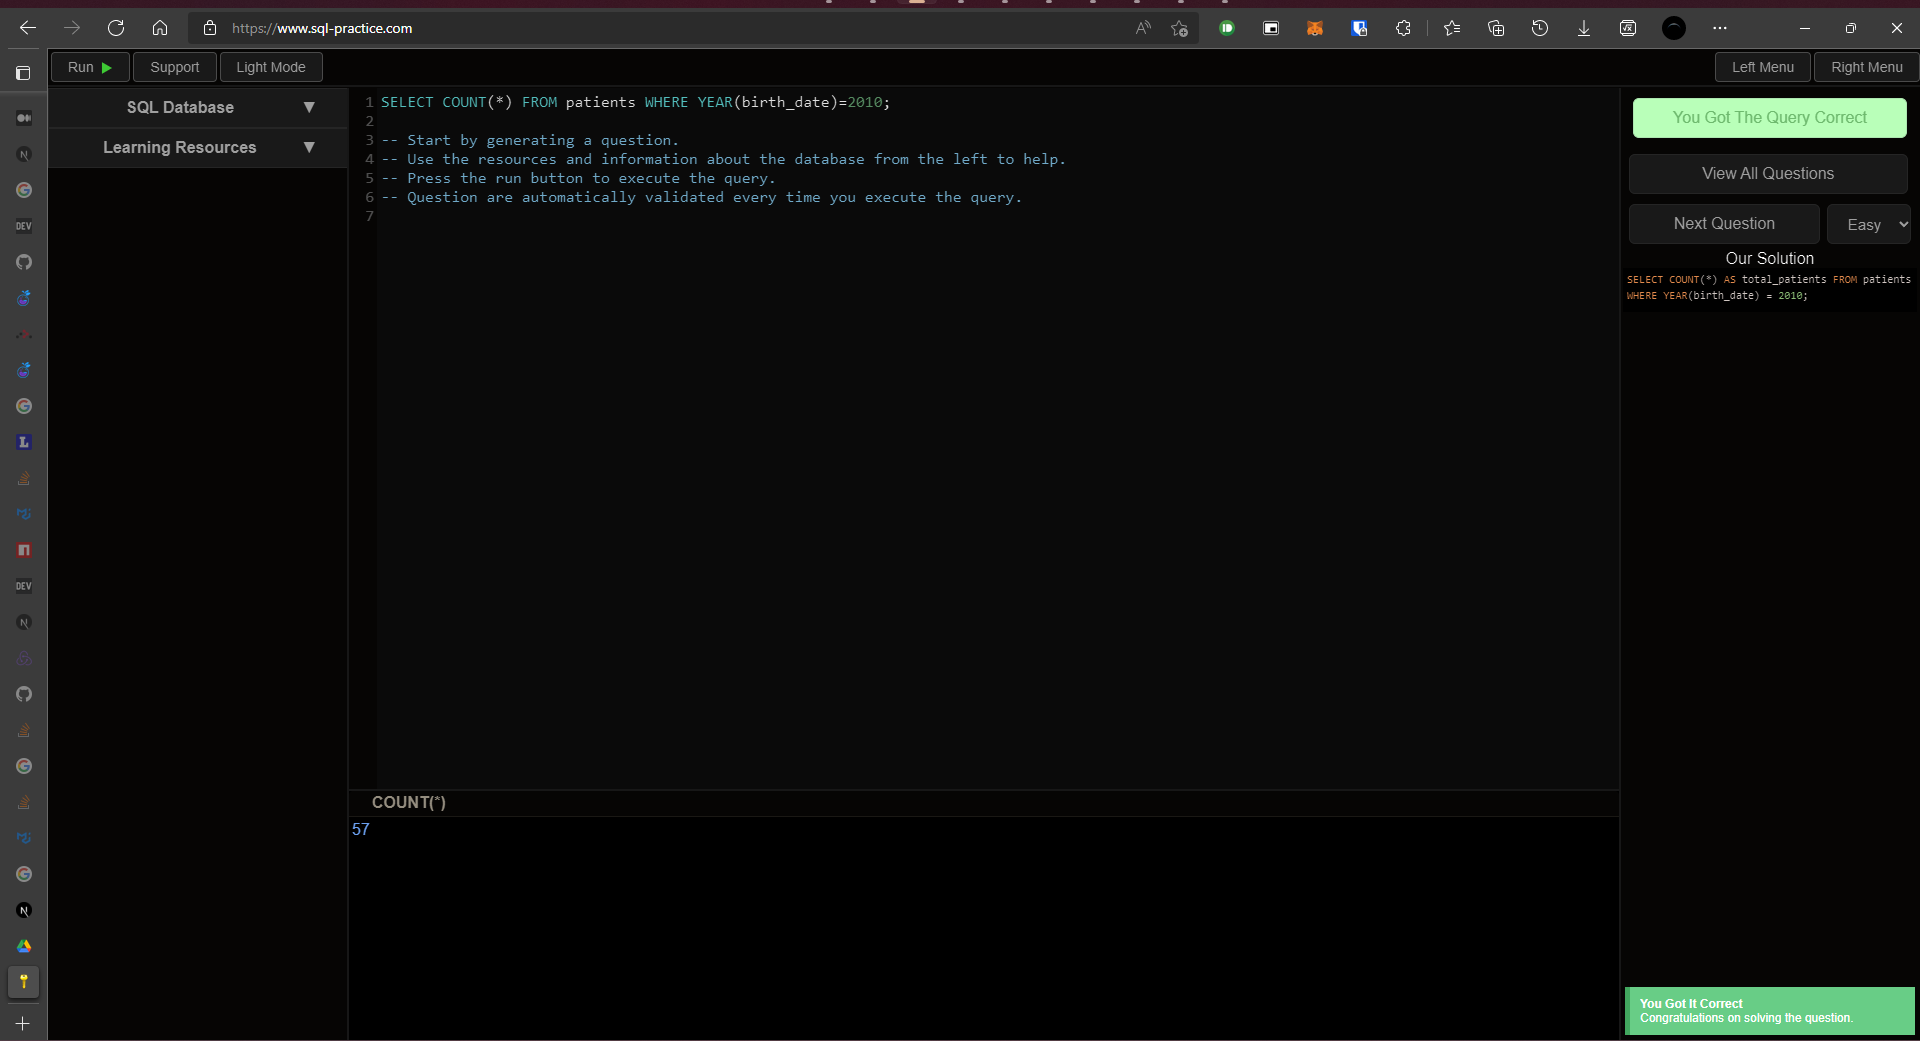
\includegraphics[width=12cm]{easy-8.png}
    \caption{Hasil Query Soal Easy 8}
\end{figure}
\subsection{Easy 9}
Show the first\_name, last\_name, and height of the patient with the greatest height.
\lstinputlisting[label={maxvalue},caption={Easy-9}, language={SQL}]{easy-9.sql}
\begin{figure}[H]
    \centering
    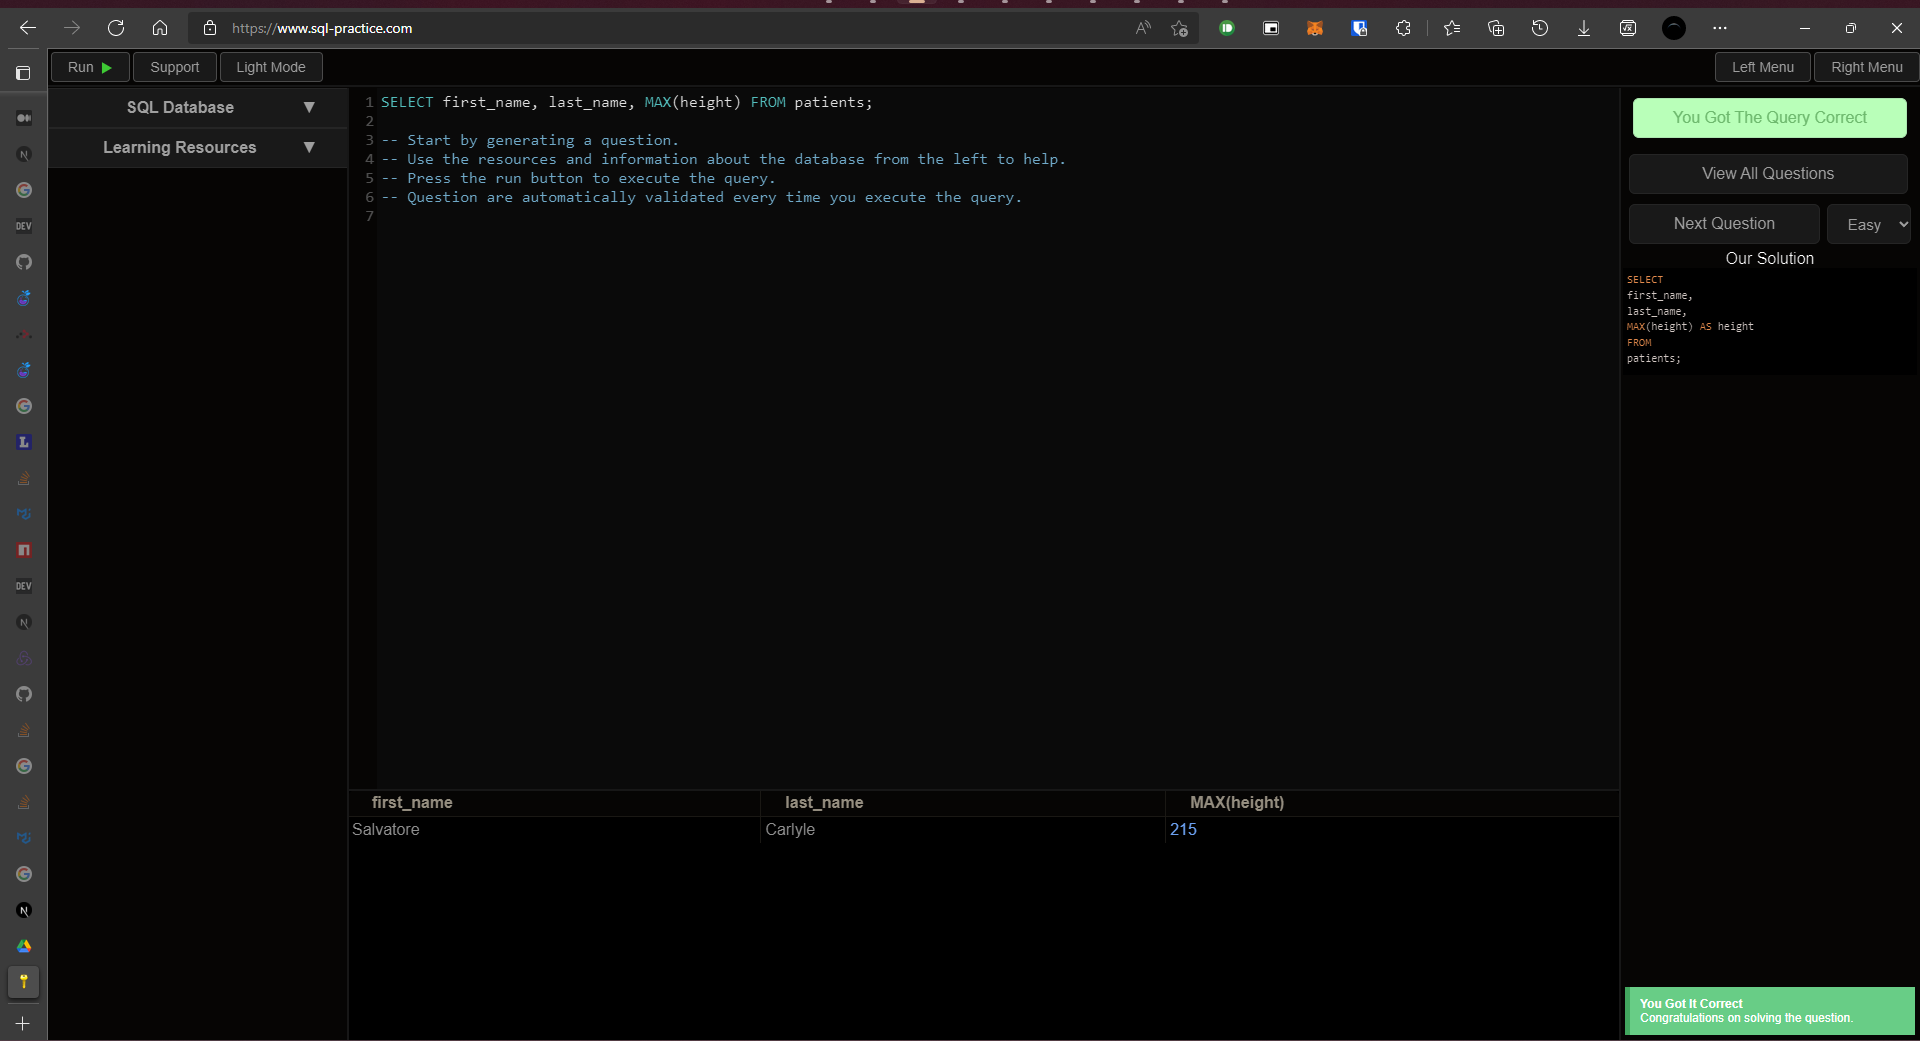
\includegraphics[width=12cm]{easy-9.png}
    \caption{Hasil Query Soal Easy 9}
\end{figure}
\subsection{Easy 10}
Show all columns for patients who have one of the following patient\_ids: 1,45,534,879,1000
\lstinputlisting[label={maxvalue},caption={Easy-10}, language={SQL}]{easy-10.sql}
\begin{figure}[H]
    \centering
    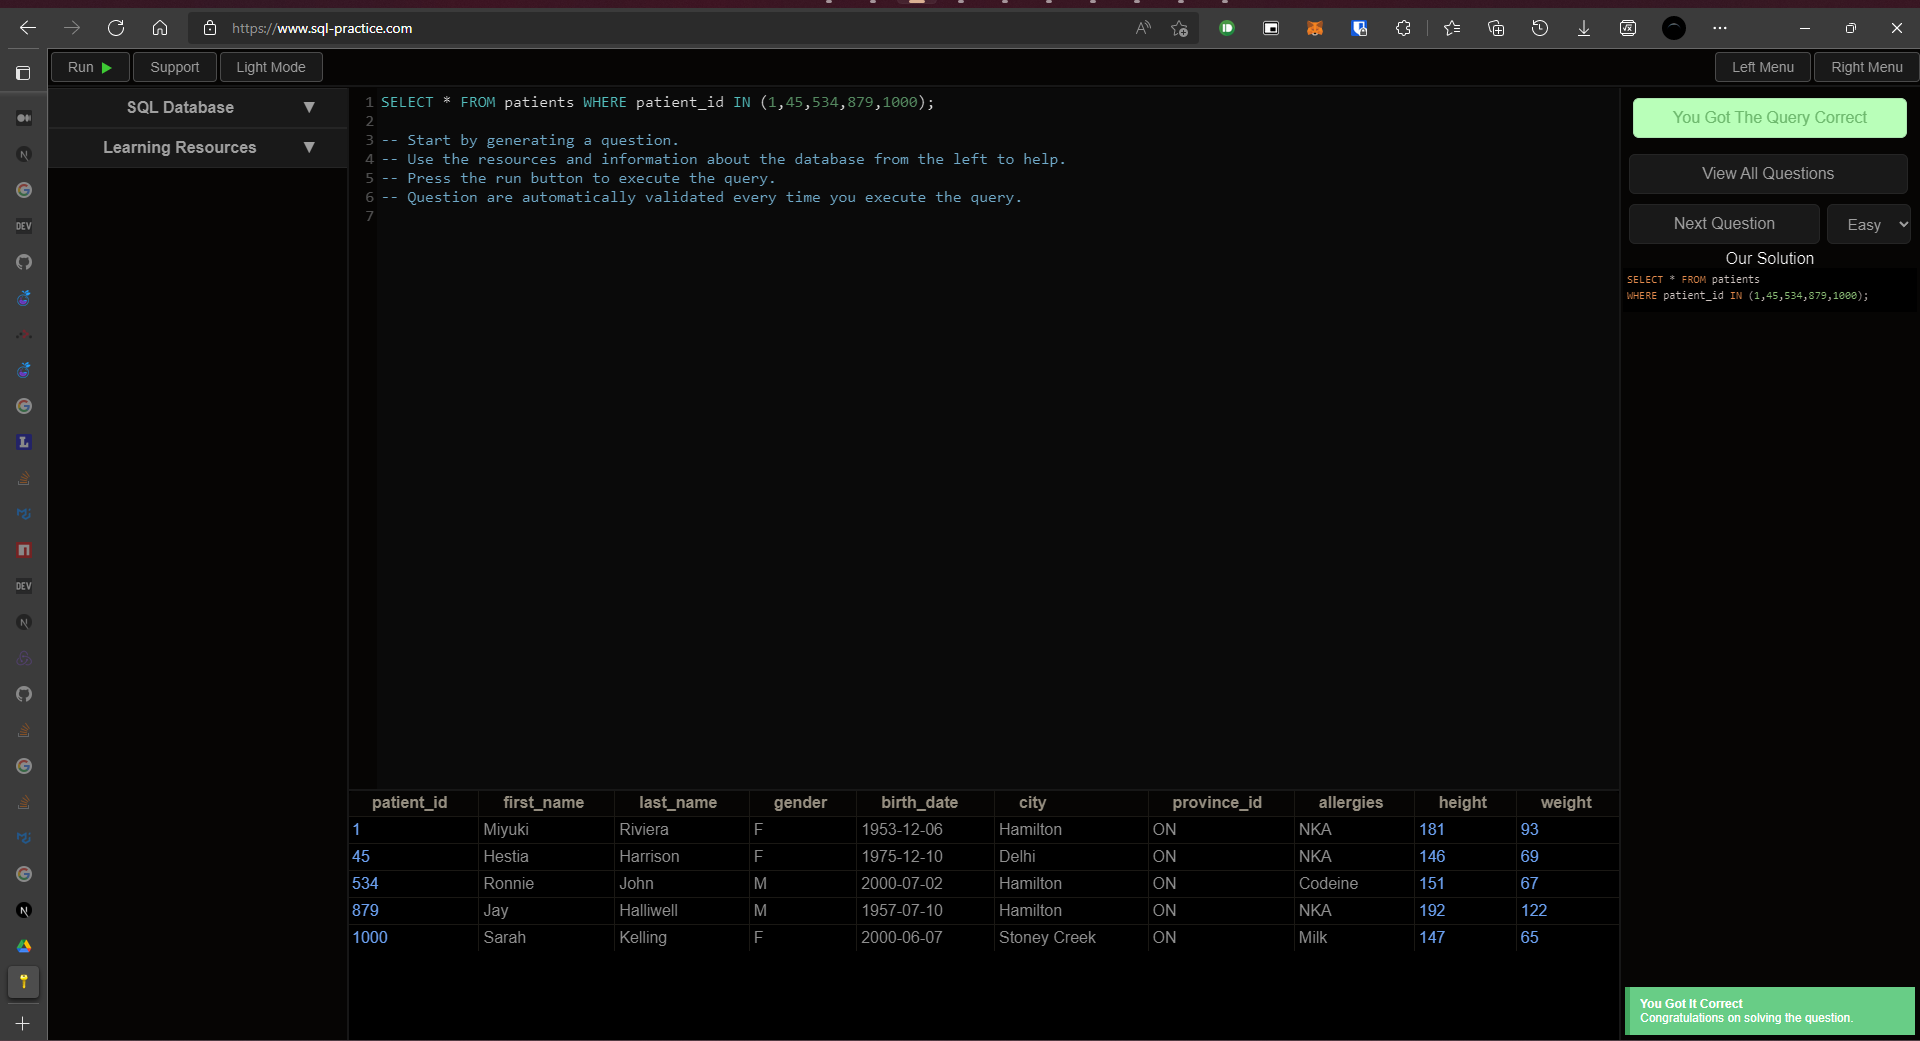
\includegraphics[width=12cm]{easy-10.png}
    \caption{Hasil Query Soal Easy 10}
\end{figure}
\subsection{Easy 11}
Show the total number of admissions

\lstinputlisting[label={maxvalue},caption={Easy-11}, language={SQL}]{easy-11.sql}
\begin{figure}[H]
    \centering
    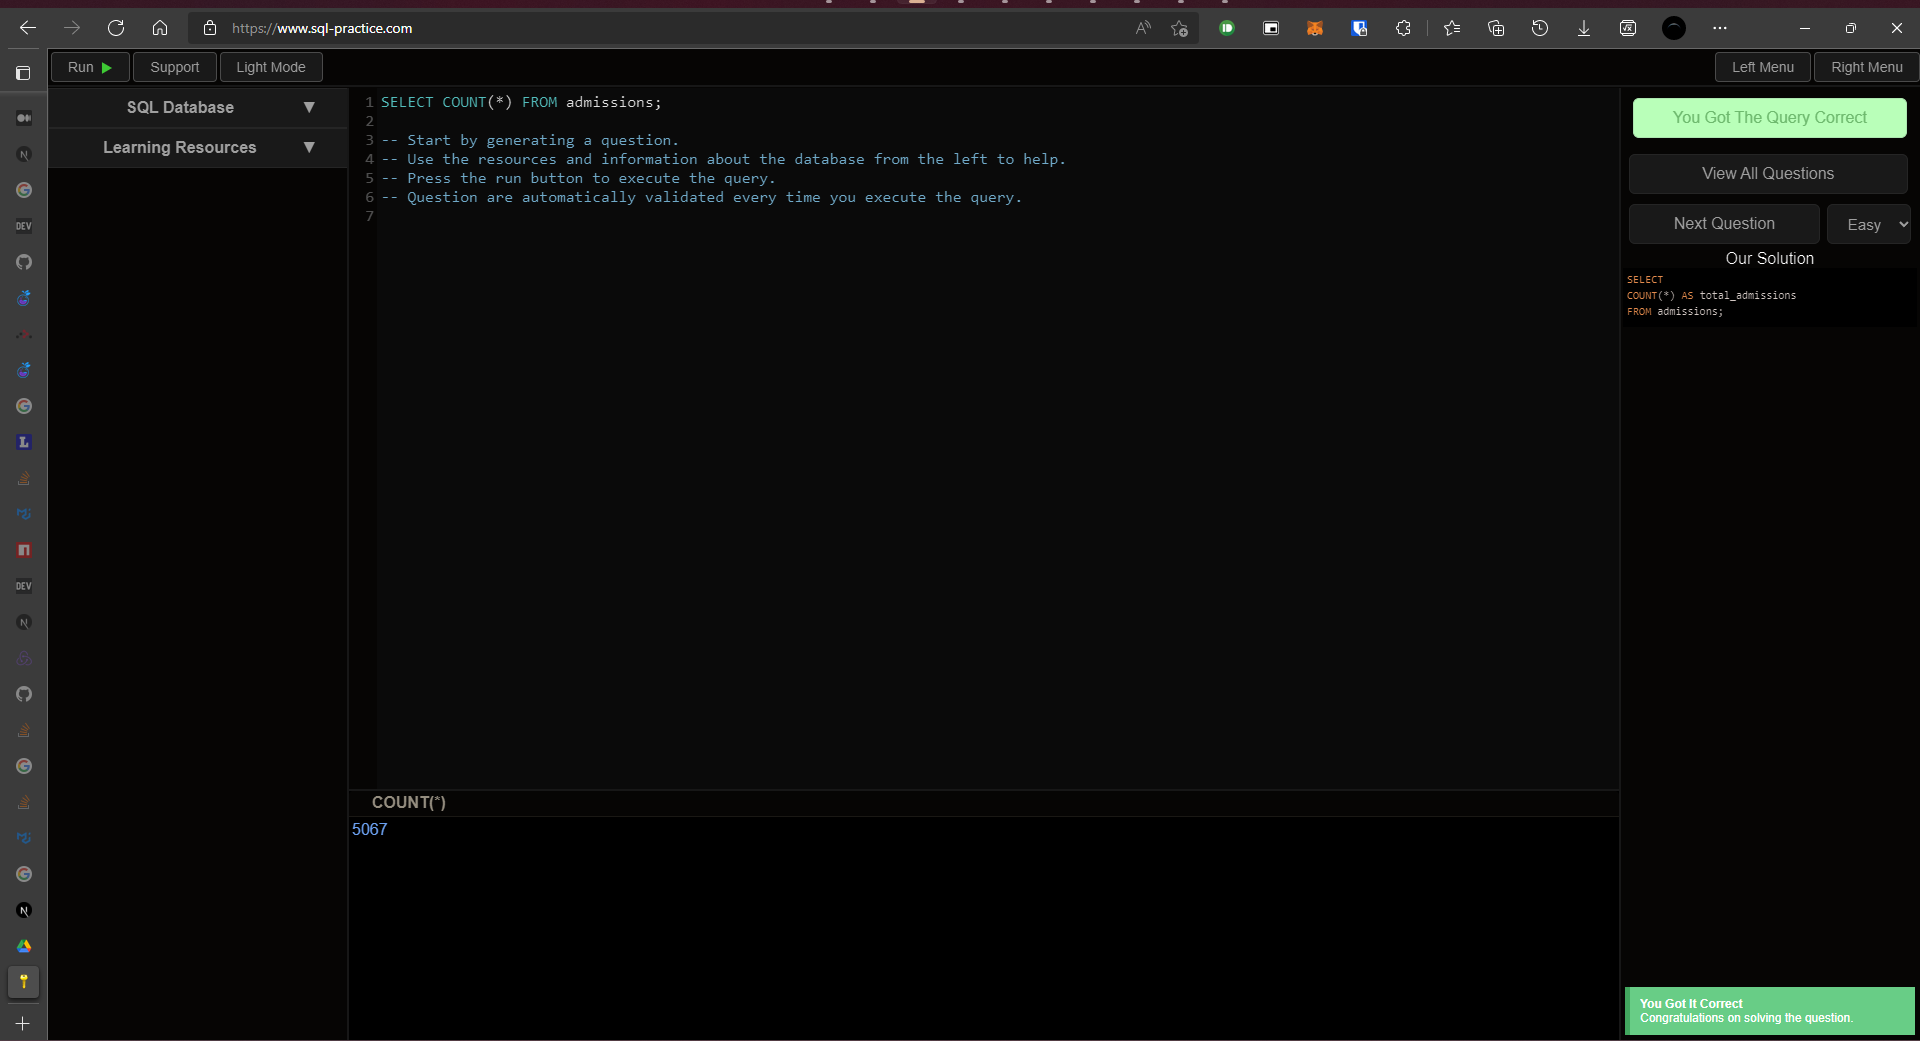
\includegraphics[width=12cm]{easy-11.png}
    \caption{Hasil Query Soal Easy 11}
\end{figure}
\end{document}